\documentclass[a4paper,12pt]{article}
\usepackage[latin1]{inputenc}
\usepackage[T1]{fontenc}
\usepackage[spanish]{babel}
\usepackage{hyperref}
\usepackage{graphicx}

\title{%

Pr\'actica 2: Limpieza y an\'alisis de los datos
	
	\author{%
	Enrique Vilanova Vidal%
		\thanks{Todos los que han colaborado en el proyecto}
	\and Brais Suarez Souto
	}
}

\begin{document}

\maketitle
\thispagestyle{empty}
\clearpage
\pagenumbering{arabic} 
\newpage

\textbf{Notas previas al ejercicio:} \\

Hemos contestado a las preguntas de acuerdo a lo indicado al ejercicio, sin embargo debido a la extensi\'on del trabajo y del c\'odigo, \'unicamente algunas partes del c\'odigo y su desarrollo  se han incluido en este texto. El objetivo es facilitar la comprensi\'on del desarrollo de las diversas partes del trabajo. El c\'odigo en su totalidad se puede encontrar en el enlace que se facilita a  \href{https://github.com/b-suarez/youtube_stats_analysis}{GitHub}.

El c\'odigo se ha hecho sobre {\itshape Google Colab} para facilitar la reproducci\'on y ejecuci\'on del trabajo. La primera parte del c\'odigo est\'a implementado en {\itshape Python} y la segunda parte en {\itshape R}. Las dos partes se han implementado sobre el mismo notebook.

En {\itshape Python} se ha implementado la limpieza general de datos, el desarrollo de m\'etricas, transformaciones exponenciales de los datos, gr\'aficas de correlaci\'on y todo lo relacionado con {\itshape Natural Language Processing}.

En {\itshape R} se ha implementado modelos de regresi\'on, an\'alisis de componente principal y test estad\'isticos.

Con el fin de aumentar la reproducibilidad del  trabajo, en el repositorio se incluyen objetos pickle y archivos csv con los datasets intermedios.

\newpage
\section[item_descripcion]{Descripci\'on del dataset. ?`Por qu\'e es importante y qu\'e  pregunta/problema pretende responder?}

\subsection{Descripci\'on del dataset.}

El conjunto de datos objeto de an\'alisis se ha obtenido a partir de este enlace en Kaggle y esta constituido por 10 datasets (uno por cada mercado regional: Canada, Alemania, Francia, Gran Breta\~na, India, Japon, Korea, M\'ejico, Rusia, Estados Unidos) de 16 caracter\'isticas (columnas) que representan los videos que han llegado a ser Trending en sus respectivas regiones.

Las caracter\'isticas representadas son las siguientes:

\begin{itemize}

\item \textbf{video{\textunderscore}id}: ID unico para cada v\'ideo.
\item \textbf{trending{\textunderscore}date}: fecha en la que el v\'ideo entr\'o en Trend.
\item \textbf{title}: T\'itulo del v\'ideo.
\item \textbf{channel{\textunderscore}title}: T\'itulo del canal al que se ha subido el v\'ideo.
\item \textbf{category{\textunderscore}id}: ID de la categor\'ia del v\'ideo. (El nombre de cada categor\'ia viene dado en un fichero json externo)
\item \textbf{publish{\textunderscore}time}: D\'ia y hora a la que se ha subido el v\'ideo.
\item \textbf{tags}: SEO tags introducidas en el v\'ideo.
\item \textbf{view}: N\'umero de visualizaciones que ha tenido el v\'ideo.
\item \textbf{likes}: N\'umero de likes.
\item \textbf{dislikes}: N\'umero de dislikes.
\item \textbf{comment{\textunderscore}count}: N\'umero de comentarios.
\item \textbf{thumbnail{\textunderscore}link}: Link d\'onde se almacena la imagen de la thumbnail.
\item \textbf{comments{\textunderscore}disabled}: Booleano que define si se han desactivado los comentarios.
\item \textbf{ratings{\textunderscore}disabled}: Booleano que define si se han desactivado los ratings.
\item \textbf{video{\textunderscore}error{\textunderscore}or{\textunderscore}removed}: Booleano que define si se han el video se ha borrado por algun error o manualmente.
\item \textbf{description}: Descripci\'on del video.

\end{itemize}

\subsection[item_importancia]{?`Por qu\'e es importante y qu\'e  pregunta/problema pretende responder?}

El dataset se ha elegido como continuaci\'on o extensi\'on de los datos recopilados en la pr\'actica 1. A modo de recordatorio, en la pr\'actica anterior nuestro objetivo era reconocer los temas que resultaban de mayor inter\'es a la mayor\'ia de la poblaci\'on en un momento en particular. Para cumplir este objetivo nos concentramos en la extracci\'on de datos de las plataformas:  {\itshape Meneame}, {\itshape Reddit} y {\itshape Twitter}. Sin embargo otra plataforma muy popular es {\itshape Youtube} de la que podemos extraer similar informaci\'on, adem\'as los atributos que obtenemos de la plataforma {\itshape Youtube} son comparables a los que obtenemos de las tres plataformas que estudiamos en la primera pr\'actica y un procesado de datos muy similar se puede establecer para los cuatro plataformas.

A partir del conjunto de datos para  {\itshape Youtube}  se plantean diferentes preguntas y an\'alisis que pueden que pueden extrapolarse f\'acilmente a los datos presentados en la primera pr\'actica. En nuestro caso hemos intentado responder a varias preguntas:

\begin{itemize}

\item  ?` qu\'e categorias son mas populares en cada mercado?
\item ?` cu\'anto tarda un video en hacerse Trending?
\item ?`Cuales son las palabras m\'s utilizadas?
\item ?`Cuales son las tags m\'as relevantes?
\item ?`Cuales son las temas m\'as importantes?
\item ?`Existen diferencias en el vocabulario que se utilizan los pa\'ises que hablan la misma lengua?
\item ?`Cual es el sentimiento y la polaridad expresada en los t\'itulos?
\item ?`Podemos modelar en n\'umero de veces que un v\'ideo se ve y establecer un modelo predictivo?

\end{itemize}

Estos an\'alisis son de gran relevancia actualmente ya que como todos sabemos, la industria de creaci\'on de contenido online genera una gran cantidad de dinero y p\'ublico. Saber navegar \'este mercado puede ser muy interesante para cualquier marca o individuo que quiera generar beneficios o atraer p\'ublico a trav\'es de YouTube.

\section{Integraci\'on y selecci\'on de los datos de inter\'es a analizar}

Tal y como se menciona en la secci\'on anterior este conjunto de datos extra\'idos de {\itshape Kaggle} cuenta con 10 datasets correspondientes a datos para la plataforma {\itshape YouTube} para diez pa\'ises diferentes. Los datasets de los diferentes pa\'ises cuentan con los mismos atributos. En general, los datsets tambi\'en presentan un fallo en la codificaci\'on de los caracteres que hace que las columnas con texto cuyos caracteres no est\'an dentro del alfabeto ingl\'es, no se cargen correctamente. Debido a esto se han seleccionado 4 datasets a tendiendo a una serie de criterios:

\begin{itemize}

\item Podemos leer entender el idioma del pa\'is donde provienen los datos. De este modo, podemos corregir problemas de codificaci\'on de caracteres en un tiempo razonable.
\item Representan zonas geogr\'aficas de varios continentes, en caso de que queramos hacer comparaciones regionales. 
\item Al menos dos datsets deben provenir de una regiones diferentes con la misma lengua. Esto permite hacer comparaciones en el uso del lenguaje.



\end{itemize} 

Atendiendo a estos criterios hemos seleccionado 4 datsets sobre  los que aplicaremos los mismo algoritmos. Todos los datos ser\'an tratados de la misma forma. En caso de que alg\'un dataset requiera un tratamiento especial en alg\'un punto se especificar\'a el motivo.

Los 4 datasets contienen datos para Alemania, Reino Unido, Mexico y EEUU.

\subsection{Descarga de datos}

Puesto que los datos ya contienen error de codificaci\'on de los atributos de texto y queremos evitar cualquier posible corrupci\'on de los datos al pasar por una m\'aquina intermedia (nuestros ordenadores), vamos a realizar una conexi\'on con Kaggle a trav\'es de su API utilizando nuestro fichero kaggle.json d\'onde guardaremos nuestras claves personales y descargamos los datos directamente a nuestro {\itshape drive} de google desde donde cargaremos los datos a nuestro notebook de {\itshape Google Colab}. 

\begin{figure}[h!]
 \centering
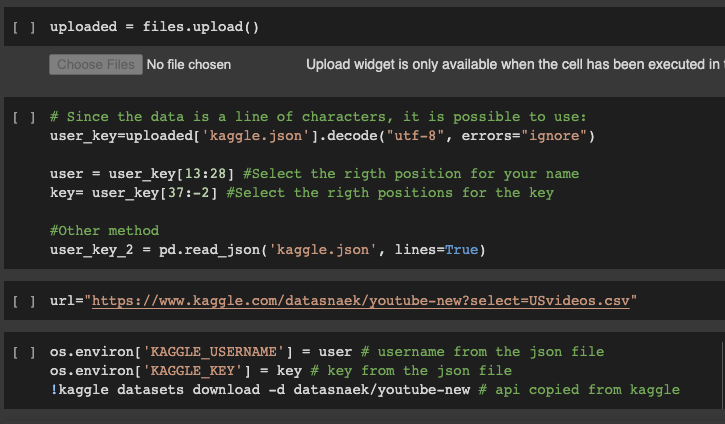
\includegraphics[width=13cm]{kaggle_upload.png}
\caption{Carga de datos desde {\itshape Kaggle}}
\label{fig:carga}
\end{figure}


Una vez nos hemos descargado los datasets y los tenemos en nuestro cloud, vamos a descomprimir el fichero y cargar los distintos datasets en un array de datasets que contendr\'a los diferentes datasets de cada mercado.
\begin{figure}[h!]
\centering
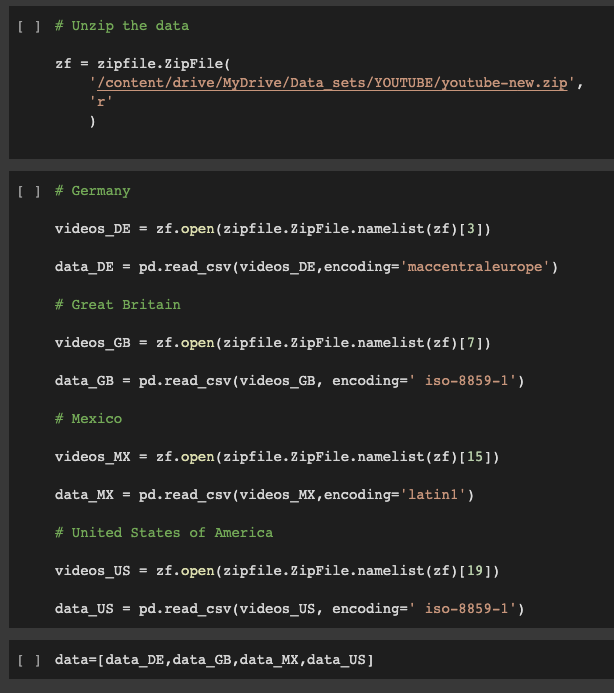
\includegraphics[width=7cm]{data_load.png}
\caption{Descomprimiendo datos desde {\itshape Google Drive}}
\label{fig:desc}
\end{figure}

\section[item_limpieza]{Limpieza de datos}

\subsection{?`Los datos contienen ceros o elementos vac\'ios? ?`C\'omo gestionar\'ias cada uno de estos casos?}

Para nuestros casos no hay valores nulos, como se puede ver en la siguiente figura\ref{fig:nula} izquierda:

\begin{figure}[h!]
\centering
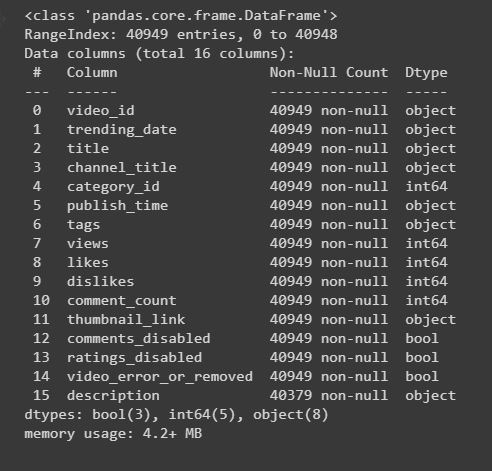
\includegraphics[width=6cm]{vacio_datos.JPG}
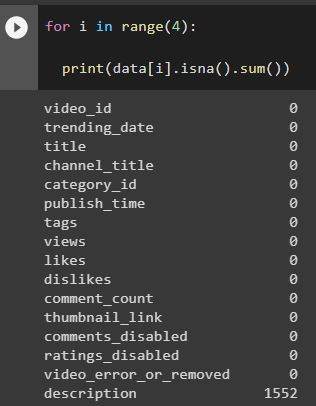
\includegraphics[width=6cm]{Na_values.JPG}
\caption{A la izquierda valores nulos. A la derecha valores {\itshape NA}}
\label{fig:nula}
\end{figure}

Los posibles elementos vac\'ios en los atributos de texto se tratan de forma separada durante la limpieza de texto.

Cuando buscamos para valores {\itshape NA} (figura \ref{fig:nula} derecha), vemos que los valores vac\'ios se encuentran en la columna {\itshape description} (atributo texto), de la que no extraemos informaci\'on en nuestro an\'alisis. A\'un as\'i, no ha habido motivo de tratar estos valores directamente ya que durante otros procesos de limpieza, las obsevaciones  que contienen {\itshape NAs} han sido eliminadas por otros motivos. Tambi\'en cabe mencionar que antes de empezar nuestro an\'alisis en {\itshape R} hemos eliminado expl\'icitamente todas las observaciones que conten\'ian valores {\itshape NA}.


\subsection{Errores en en los c\'odigos de tiempo}

Una de las primeras errores que hemos podido detectar es que los datos referentes a c\'odigos de tiempo se encontraban en formatos diferentes. Por lo que se ha unificado los formatos de tiempo y convertirlos datos de {\itshape object} a {\itshape datetime}.

\subsubsection{Correcci\'on  trending date}

Transformaci\'on de todas las columnas que contengan un valor de fecha a tipo datetime, empezando por la columna trending date.

\begin{figure}[h!]
 \centering
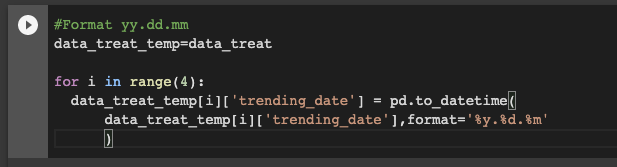
\includegraphics[width=13cm]{correc_trending.png}
\caption{Conversi\'on para {\itshape trending date}}
\label{fig:trend_date}
\end{figure}

\subsubsection{Correcci\'on  publish time}
Vamos a realizar la misma operaci\'on con la columna publish time.

\begin{figure}[h!]
\centering
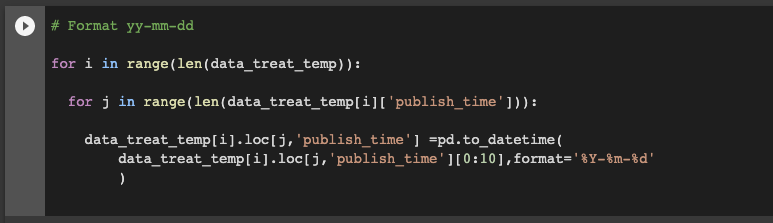
\includegraphics[width=13cm]{correc_publish.png}
\caption{Conversi\'on para {\itshape publish time}}
\label{fig:pub_date}
\end{figure}


\subsection{Correcci\'on  textos}
La parte de {\itshape language cleaning} es muy importante para nuestro proyecto, ya que tener textos limpios y analizables nos ser\'a \'util para futuros   an\'alisis.


\subsubsection{Limpieza general}

En nuestro caso hemos definido diferentes funciones para corregir caracteres mal codificados, emoticonos, signos de puntuaci\'on que no necesitamos para el an\'alisis del lenguaje natura, as\'i como una funci\'on espec\'ifica para tratar carateres especiales del alfabeto alem\'an l. Hemos aplicado a las columnas: title, channel{\textunderscore}title,  tags y description. Las funciones se presentan el figura \ref{fig:corrtext}.



\begin{figure}[h!]
\centering
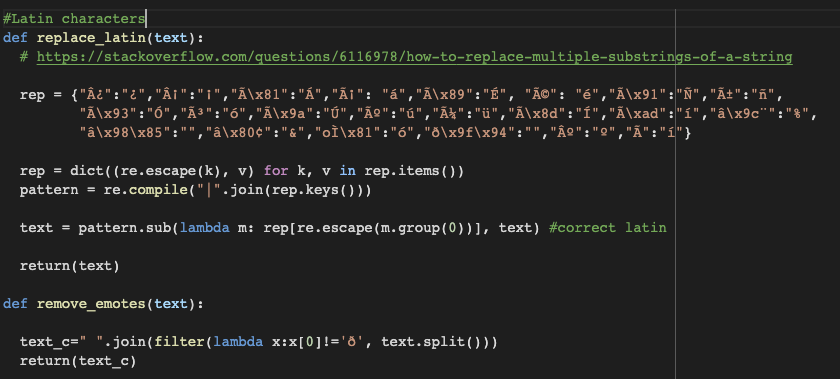
\includegraphics[width=10cm]{latin_characters.png}\\
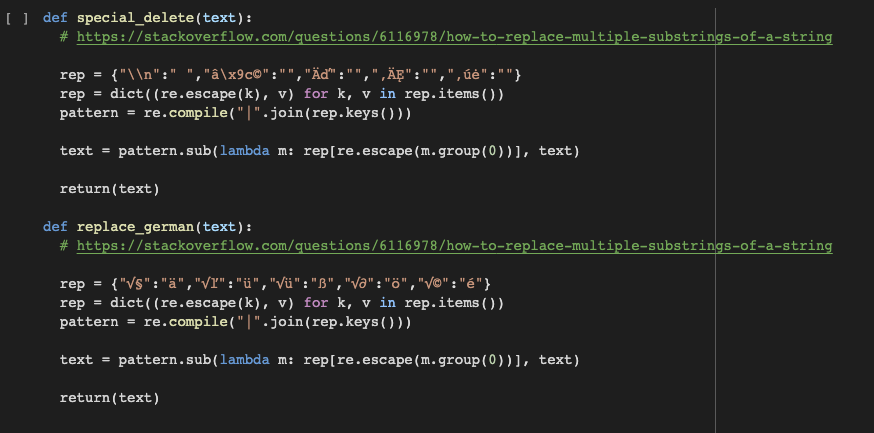
\includegraphics[width=10cm]{german_characters.png}\\
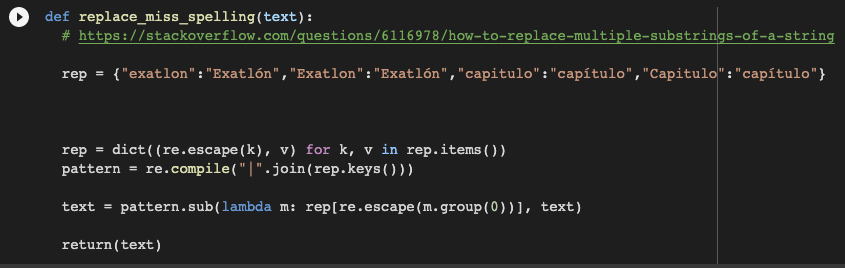
\includegraphics[width=10cm]{misspellings.png}
\caption{Correci\'on de texto}
\label{fig:corrtext}
\end{figure}

A de m\'as de las correcciones presentadas han sido necesarias, varias rondas de correci\'on de texto donde se han eliminado errores que no se hab\'ian capturado inicialmente. Todo esto se puede ver dentro del c\'odigo en la secci\'on {\itshape Some NLP-More Cleaning}

\subsubsection{{\itshape Stop Words} para el {\itshape document-Term Matrix}}

Con el fin de realizar las {\itshape World Clouds}, hay que eliminar del {\itshape document-Term Matrix} todas las {\itshape Stop Words}. El m\'odulo {\itshape Count Vectorizer} de {\itshape sklearn} ya proporciona una lista de {\itshape Stop Words} para ingl\'es pero debe ampliarse para otros lenguajes. De proyectos anteriores, ya dispon\'iamos de listas de {\itshape Stop words} para otros idiomas, que hemos a\~nadido, como se puede ver en la figura \ref{fig:stop}.

\begin{figure}[h!]
\centering
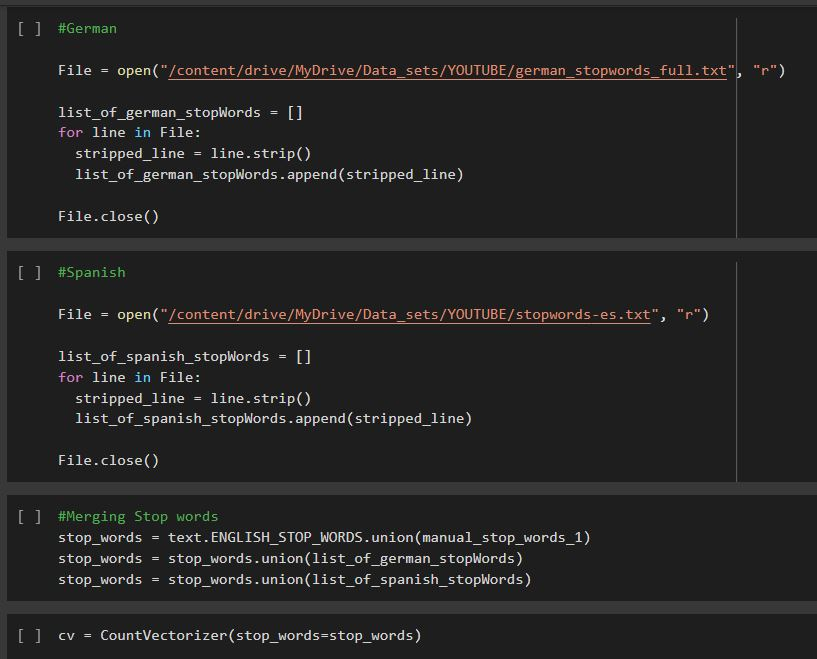
\includegraphics[width=10cm]{Stop_words.JPG}\\
\caption{A\~nadiendo {\itshape Stop Words}}
\label{fig:stop}
\end{figure}

A de m\'as de estas {\itshape Stop Words} ha sido necesario a\~nadir manualmente m\'as palabras debido a los errores de codificaci\'on de los textos

\subsection{Identificaci\'on y tratamiento de valores extremos}

Para nuestro caso los valores extremos en visitas o cuentas de comentarios marcan los v\'ideos m\'as populares, por lo que no parece acertado tratar estos datos como si de errores se tratasen, ya que estos valores extremos nos pueden indicar casos interesantes de estudio. por otra parte, al estudiar cuanto tiempo tarda un v\'ideo en convertirse  en tendencia, hemos visto que hay v\'ideos que pueden tardar hasta once a\~nos en llegar a tendencia. Estos caso, si son outliers  para nosotros. Nuestro caso de estudio es, como las cosas que ocurrieron ayer afecta a los que ser\'a tendencia ma\~nana y cuanto dura el impacto de estos hechos en el tiempo. Despu\'es de analizar las deltas de tiempo hemos considerado razonable eliminar cualquier video que tarde m\'as de 40 d\'ias en convertirse en tendencia por dos razones; Si algo tarda m\'as de 40 d\'ias en convertirse en tendencia no proviene de v\'ideos de historias recientes. Los v\'ideos que tardan m\'as de 40 d\'as en convertirse en tendencia suponen menos del $1.5\%$ de la informaci\'on total. En la figura \ref{fig:delta} se presenta la m\'etodo de eliminaci\'on de estos datos.

\begin{figure}[h!]
\centering
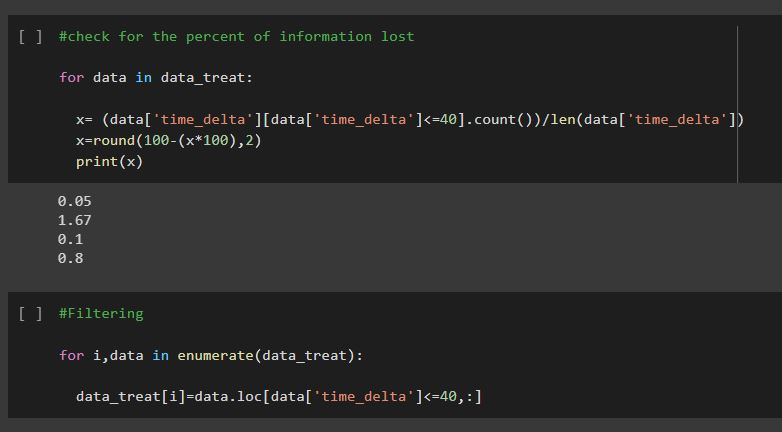
\includegraphics[width=10cm]{tiempo.JPG}\\
\caption{Eliminamos las observaciones con una delta de tiempo superior a 40 d\'ias y se comprueba la cantidad de informaci\'on perdida}
\label{fig:delta}
\end{figure}

\section{An\'alisis de los datos}

\subsection{Selecci\'on de los grupos de datos que se quieren analizar/comparar (planificaci\'on de los análisis a aplicar).}

\subsubsection{V\'ideos con defectos}

De entre todas las columnas destacan unas con valores l\'ogicos:  {\itshape commentsdisabled}, {\itshape ratingsdisabled} y {\itshape video error or removed}, que est\'an marcados indicando alg\'un tipo de carencia. Con el fin de homogeneizar los datos, es decir, hacer que todos nuestros datos provengan de v\'ideos con las mismas caracter\'isticas generales, vamos a eliminar las filas con valores {\itshape True} en cualquiera de estos atributos. Esto se puede ver en la figura \ref{fig:defect}. Tambi\'en se puede observar que en general se conserva m\'as del $96\%$ de la informaci\'on. 


\begin{figure}[h!]
\centering
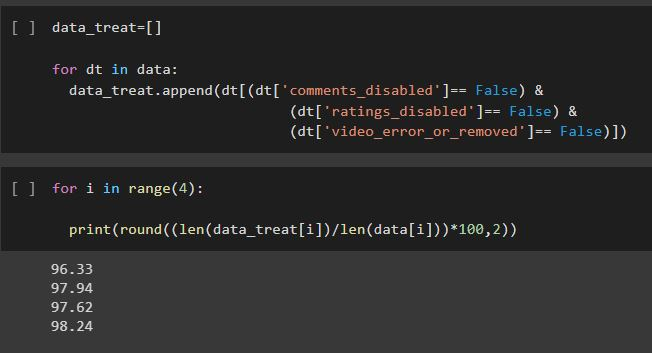
\includegraphics[width=13cm]{data_selection_2.JPG}
\caption{Eliminamos las v\'ideos con defectos y comprobamos cuanta informaci\'on se conserva}
\label{fig:defect}
\end{figure}




Debido a que estas columnas solo contienen valores {\itshape FALSE} despu\'es de elimar los {\itshape TRUE}, ya no es relevante conservar estas columnas por lo que se eliminan (esto se puede ver en c\'odigo en la secci\'on {\itshape data cleaning}).

\subsubsection{Eliminamos categor\'ia sin informaci\'on (category = 29)}

No existe informaci\'on sobre que categir\'ia representa el id 29, por lo tanto eliminamos \'esta del dataset. Otra raz\'on para eliminarla es que al no saber que representa dicha categor\'ia, aun en el caso que pudi\'esemos extraer alguna informaci\'on para la categor\'ia 29, no podr\'iamos darle un sentido concreto

En la figura \ref{fig:cat29}, se puede ver que despu\'es de eliminar los observaciones de esta categor\'ia, preservamos m\'as del 95 porciento de la informaci\'on.

\begin{figure}[h!]
\centering
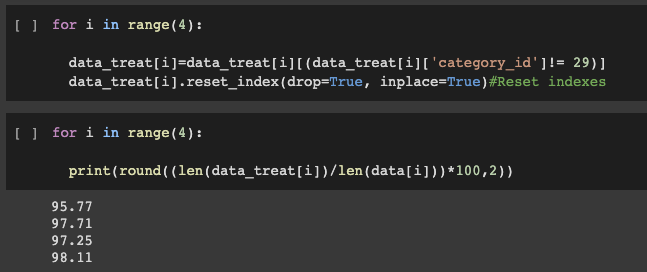
\includegraphics[width=13cm]{remove_category.png}
\caption{Eliminamos la categor\'ia 29 y comprobamos el porcentaje de informci\'on conservada}
\label{fig:cat29}
\end{figure}





\subsubsection[item_metricas]{Generaci\'on de m\'etricas y an\'alisis de datos}

Nuestros datos en bruto pueden carecer de sentido sin una referencia; ?`Son dos v\'ideos con el mismo n\'umero de visitas igual de relevantes? o Para dos videos con el mismo n\'umero de likes, ?`Podemos pensar que han despertado el mismo inter\'es?. otro ejemplo ser\'ia tenemos videos con un gran n\'umero de visitas pero pocos comentarios (lo que llamariamos un click bait), o un video con pocas visitas pero un gran n\'umero de comentarios.

Para poder solventar inconveniente de que carecemos de referencias y poder analizar correctamente los v\'ideos, creamos una serie de m\'etricas relativas que nos ayudar\'an a realizar an\'alisis m\'as  de los v\'ideos.

\textbf{Sentimiento relativo:} \\
La m\'etrica {\itshape relative video sentiment} (rvs) se calcula utilizando la f\'ormula {\itshape (likes-dislikes)/sum(likes+dislikes)} y nos ayudar\'a a hacernos una idea de el sentimiento que genera un video sobre 1. Si el sentimiento que genera el v\'ideo es positivo el valor de rvs ser\'a positivos y si tiene m\'as {\itshape dislikes} el valor de rvs ser\'a negativo. Se puede ver expl\'icitamente el proceso seguido en la figura \ref{fig:rvsform}

\begin{figure}[h!]
\centering
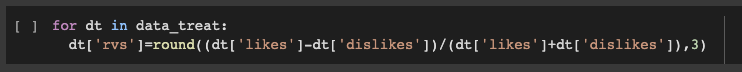
\includegraphics[width=13cm]{rvs_gen.png}
\caption{Ecuaci\'on para generar rvs}
\label{fig:rvsform}
\end{figure}

Haciendo un plot de las frecuencias obtenidas sobre esta m\'etrica, nos damos cuenta de que los videos que llegan a ser {\itshape trending}, tienden a tener m\'as {\itshape likes} que {\itshape likes}. De hecho la mayar\'ia de v\'ideos que llegan a {\itshape ttrending} tienen al menos un $75\%$ de {\itshape likes} frente a {\itshape dislikes}. Esto se puede ver en la figura \ref{fig:rvsgraf}.

\begin{figure}[h!]
\centering
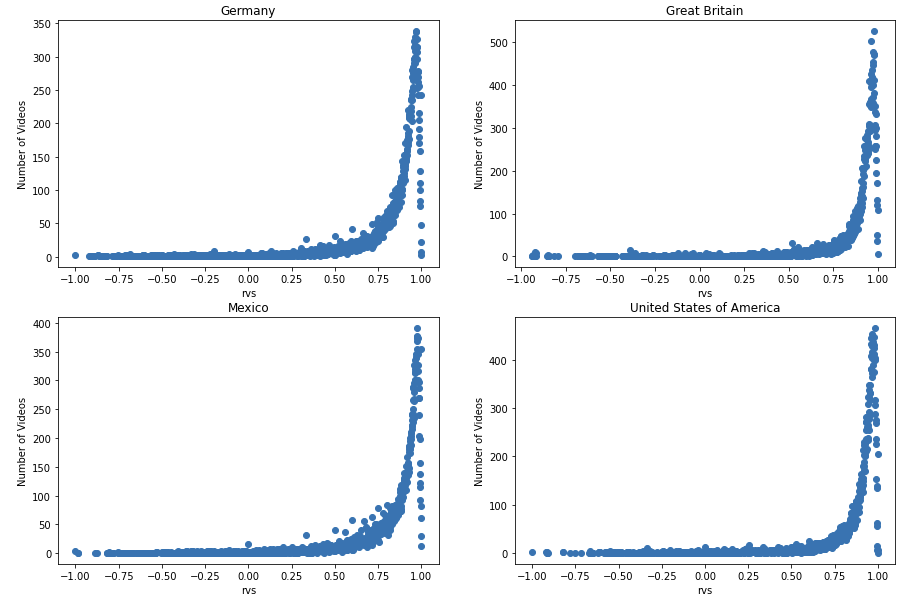
\includegraphics[width=14cm]{rvs_plot.png}
\caption{N\'umero de ocurrencias por rvs}
\label{fig:rvsgraf}
\end{figure}

\textbf{M\'etrica relevancia:}\\
Sabemos que para los usuarios comentar un video conlleva m\'as esfuerzo que hacer click a {\itshape like} o {\itshape dislike}. Tambi\'en entendemos que un video tiene mayor cantidad de comentarios cuando los viewers tienen algo que decir sobre el tema o alg\'un comentario a provocado controversia.

Para medir esto, hemos creado un atributo {\itshape rel{\textunderscore}elevance}, el cual se calcula con la formula {\itshape comment{\textunderscore}count/(likes+dislikes)}. Cuando su valor tiende a 1 asumimos que el video es relevante para los {\itshape viewers} y cuando es mayor que 1 quiere decir que es muy relevante. la geberaci\'on de la m\'etrica se puede ver la figura \ref{fig:relfor}.
\begin{figure}[h!]
\centering
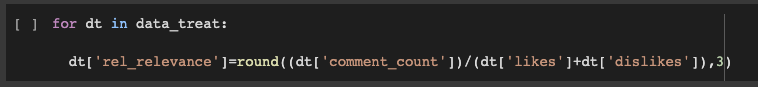
\includegraphics[width=13cm]{rel_gen.png}
\caption{Ecuaci\'on para generar la m\'etrica de relevancia relativa}
\label{fig:relfor}

\end{figure}

Haciendo un plot de las frecuencias de este valor (figura \ref{fig:relfig}), podemos observar que la mayor parte de los videos tiene un valor menor que  1.  De hecho, observamos que los v\'ideos que alcanzan{\itshape trending} tienen a tener un ratio menor que 0.5, alcanzando un pico claro alrededor 0.25.

Esto nos da a entender que los v\'ideos que alcanzan {\itshape trending} no suelen ser muy pol\'emicos en general, lo cual tiene sentido ya que suelen ser v\'ideos que atraen a un p\'ublico general.

\begin{figure}[h!]
\centering
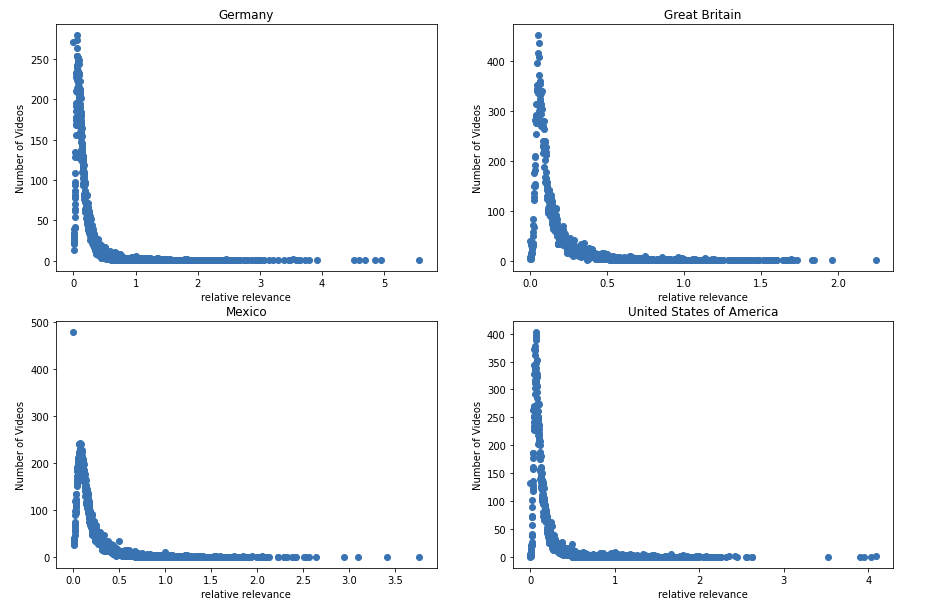
\includegraphics[width=14cm]{rel_relevance_plot.png}
\caption{N\'umero de ocurrencias para la relevancia relativa}
\label{fig:relfig}

\end{figure}

\textbf{M\'etrica sentiment engagement:}

Por \'ultimo vamos a generar 3 atributos relacionados con el{\itshape sentiment engagement} de los v\'ideos, estos ser\'an el {\itshape positive engagement}, {\itshape negative engagement} y {\itshape overall engagement}.
\newpage
Estas m\'etricas se calculan como: \footnote{Los c\'alculos se han realizado de la misma forma que se ha mostrado en la dem\'as m\'etricas. Los detalles pueden verse en el notebook, apratdo m\'etricas.}

\begin{itemize}
\item {\itshape Positive engagement} se calcular\'a utilizando la f\'ormula: {\itshape likes/views}


\item {\itshape Negative engagement} se calcular\'a utilizando la f\'ormula: {\itshape dislikes/views}



\item {\itshape Overall engagement} se calcular\'a utilizando la f\'ormula: {\itshape (likes-dislikes)/views}

\end{itemize}

Al representar sus frecuencias (figura \ref{fig:rengan}) podemos ver que los v\'ideos {\itshape trending} tienen un n\'umero de {\itshape likes} o {\itshape dislikes} muy peque\~no en comparaci\'on con las visualizaciones. De hecho la mayor\'ia  de ellos apenas tienen un $10\%$ de {\itshape likes} en comparaci\'on con las views. Y la mayor\'ia de las views son {\itshape likes}. Esto \'ultimo es m\'as evidente en la curva  para {\itshape Overall engagement} que para todos los casos, est\'a m\'as desplazada hacia el lado de los valores positivos.


\begin{figure}[h!]
\centering
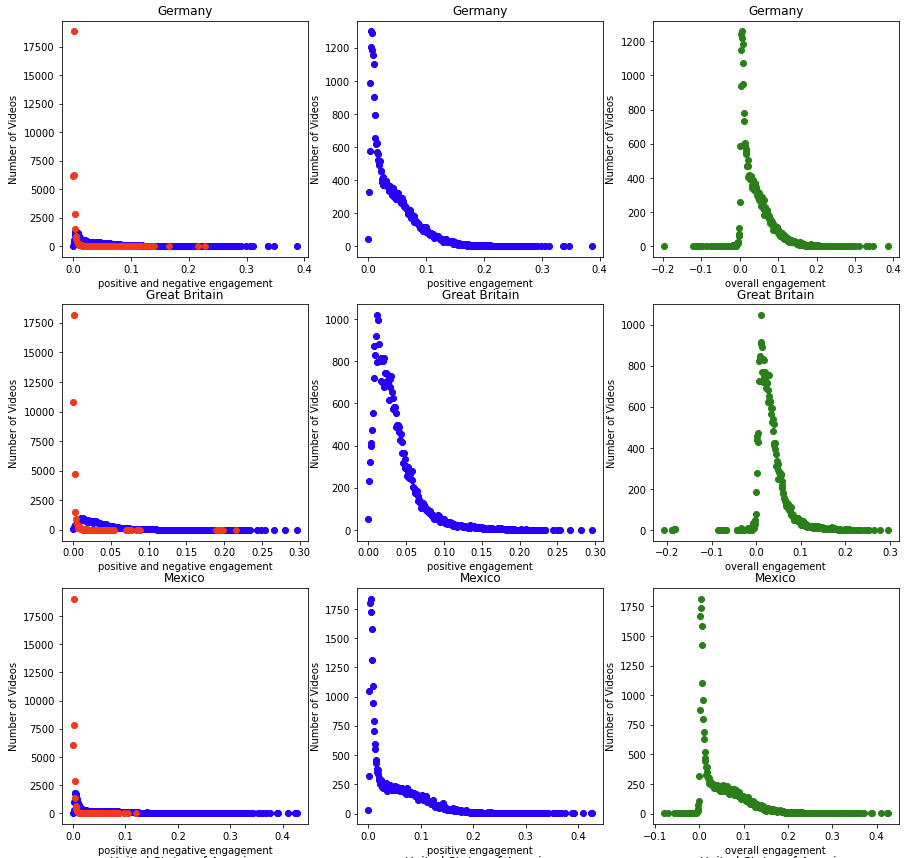
\includegraphics[width=13cm]{engagement_1.png}
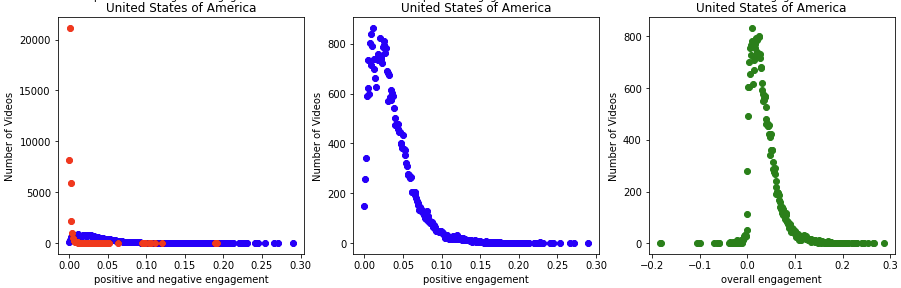
\includegraphics[width=13cm]{engagement_2.png}
\caption{N\'umero de ocurrencias para cada {\itshape sentiment engagement}}
\label{fig:rengan}
\end{figure}

\subsection{Comprobaci\'on de la normalidad y homogeneidad de la varianza.}

Nuestro daset presenta dos dificultades a la hora de comprobar si los datos y las m\'etricas siguen una distribuci\'on normal. Por una parte el gran n\'umero de datos hace inviable la aplicaci\'on del test de normalidad de {\itshape  Shapiro Wilk}, por otra parte, al existir muchos valores repetidos para un atributo el test de {\itshape Anderson Darling} no es fiable ya que siempre devolver\'a como resultado el rechazo de la hip\'otesis nula. Por este motivo nos centramos en los valores de {\itshape Kurosis} y {\itshape Skewness}. Para estos test, t\'ipicamnete se considera que una distribuci\'on es normal cuando el valor de {\itshape Kurtosis} est\'a entre $-2$ y $+2$ y para {\itshape skewness} los valores deben caer dentro del intervalo entre $-0.8$ y $+0.8$.

Hemos creado una funci\'on {\itshape normal check} que nos devuelve 1 cuando los datos de un atributo siguen una distribuci\'on normal (en las condiciones especificadas arriba) y 0 cuando no la sigue. La hemos aplicado sobre todas las columnas de todas los datasets y los datos los hemos visualizado como un dataframe que se copia abajo (los detalles de la funci\'on se encuentran el notebook).

Podemos comprobar que tanto los valores de los datos en crudo, como las m\'etricas que hemos implementado no siguen una distribuci\'on normal (figura \ref{fig:norm_1}). Con el fin de solucionar este problema y conseguir una distribuci\'on homogenea de la varianza, hemos optado por utilizar en primera instancia una transformaci\'on de {\itshape Yeo Jhonson}, puesto que nos permite aplicar el mismo c\'odigo sobre todos los atributos (una transformaci\'on de {\itshape Yeo Jhonson} a diferencia de {\itshape Boxcox} nos permite trabajar con valores negativos y ceros).




\begin{figure}
\centering
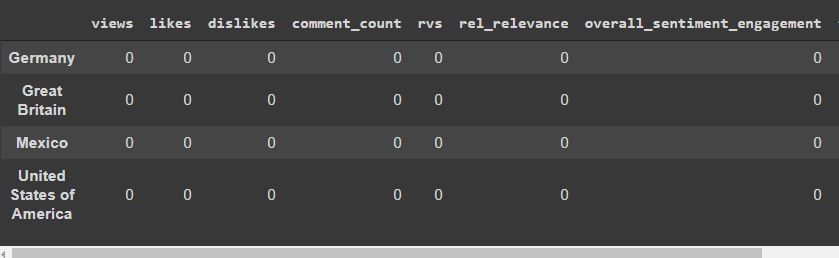
\includegraphics[width=12cm]{dataframe_1.JPG}
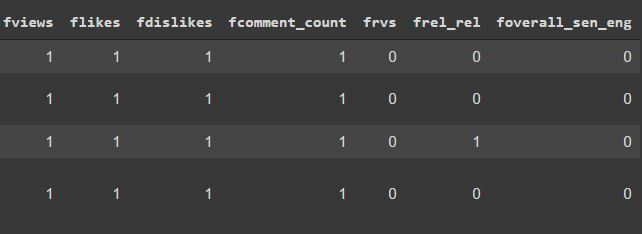
\includegraphics[width=12cm]{dataframe_2.JPG}
\caption{Comprobaci\'on de normalidad}
\label{fig:norm_1}
\end{figure}
 
Como se puede ver los datos en crudo se han podido transformar de forma que ahora siguen una distribuci\'on normal (figura \ref{fig:norm_1}). Los datos transformados se guardan en las columnas {\itshape fviews}, {\itshape likes}, {\itshape dislikes} y {\itshape fcommentl{\textunderscore}count}. Adem\'as los valores de lambda tambi\'en se guardan para poder deshacer la transformaci\'on (se pueden ver todos los detalles en el notebook en el apartado {\itshape Power transformation and descriptive statistics for the metrics}).

Sin embargo, las m\'etricas no siguen todav\'ia una distribuci\'on normal. Intentamos corregir este hecho hemos realizado una transformaci\'on por quantiles sobre las m\'etricas. Los nombres asociados a los datos de las m\'etricas trasnformados por quartiles son : {\itshape q{\textunderscore}rvs}, {\itshape q{\textunderscore}rel{\textunderscore}rel} y{\itshape q{\textunderscore}overall{\textunderscore}sen{\textunderscore}eng}. Una vez hechas las transformaciones, volvemos aplicar la funci\'on implementada para el c\'alculo de la normalidad de los atributos y representamos los resultados en un dataframe que se puede ver en la figura \ref{fig:quar}.

\begin{figure}[h!]
\centering
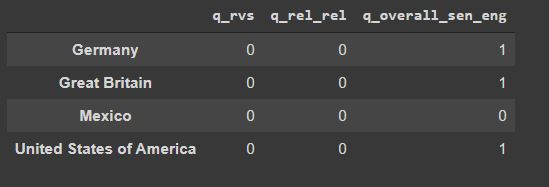
\includegraphics[width=12cm]{dataframe_3.JPG}
\caption{Transformaci\'on por quartiles para las m\'etricas}
\label{fig:quar}
\end{figure}

Se ve una discrepancia en los datos de {\itshape M\'exico}. Hacemos un gr\'afico de densidades para la los datos {\itshape q\_overall\_sen\_eng}, es decir los datos que cuya variable  ha sufrido una transformaci\'on por quantiles.

\begin{figure}[h!]
\centering
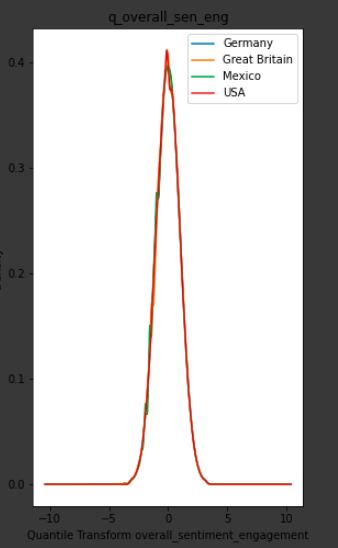
\includegraphics[width=5cm]{grafica_transformada.JPG}
\caption{G\'afico de densidades para {\itshape q{\textunderscore}overall{\textunderscore}sen{\textunderscore}eng}}
\label{fig:quart_2}
\end{figure}

En la curva de la figura \ref{fig:quart_2}, no podemos apreciar ninguna diferencia significativa entre las curvas para cada pa\'is.

En conclusi\'on ahora contamos con los datos transformados  v\'ia {\itshape Yeo\-Jhonson} que siguen una distribuci\'on normal y la m\'etrica {\itshape overall\_sent\_eng} que transformada por quartiles tambi\'en sigue una distribuci\'on normal por lo que podremos aplicar test de correlaci\'on, modelos de regresi\'on y otros test estad\'isticos para m\'etricos.

Como nota final tambi\'en se ha investigado la normalidad de las deltas de tiempo y su distribuci\'on no es normal. Pero se ha podido alcanzar una distribuci\'on normal usando transformaciones exponenciales (el c\'odigo con los c\'alculos se encuentran en el notebook; apartado {\itshape How long does it take for a Video to get trending?} sub apartado {\itshape power transformation}).

\subsection[item_pruebas]{Aplicaci\'on de pruebas estad\'isticas para comparar los grupos de datos. En funci\'on de los datos y el objetivo del estudio, aplicar pruebas de contraste de hip\'otesis, correlaciones, regresiones, etc. Aplicar al menos tres m\'etodos de an\'alisis diferentes.}


\subsubsection{M\'etodo 1: Correlaci\'on}

Una vez normalizado los datos podemos aplicar el m\'etodo de correlaci\'on de {\itshape Pearson}. En la figura \ref{fig:corrplot} es interesante ver que los atributos transformados presentan una alta correlaci\'on. Si ahora nos fijamos en los atributos sin transformar esta correlaci\'on aunque alta no es tan marcada como en los atributos transformados.  La alta correlaci\'on tambi\'en apunta al hecho que es factible esperar encontrar una relazi\'on lineal entre atributos transformados.
 
\begin{figure}[h!]
\centering
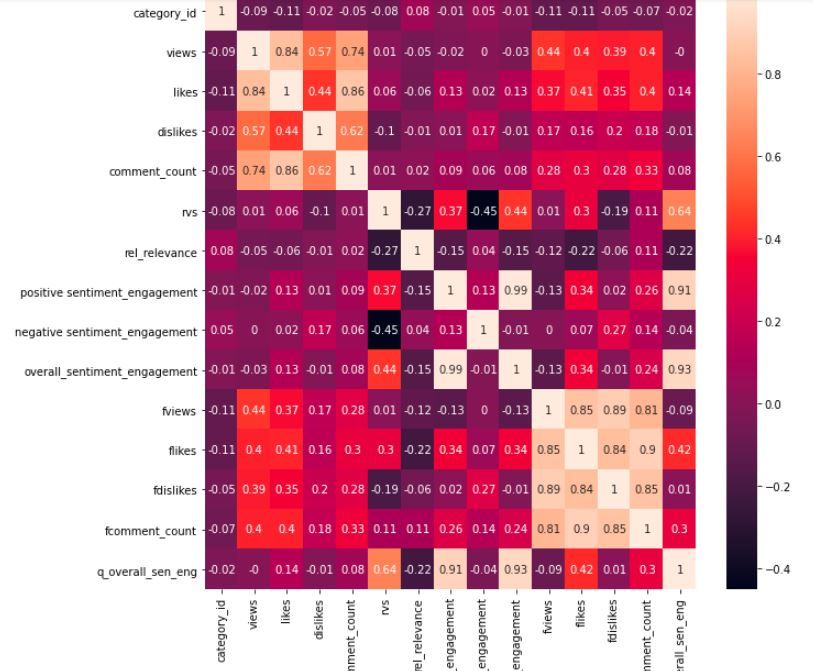
\includegraphics[width=10cm]{Correlation.JPG}
\caption{G\'afico de correlaciones para todos los atributos}
\label{fig:corrplot}
\end{figure}

\subsubsection{M\'etodo 2: Modelos de regresi\'on}

En este punto nuestro objetivo es construir un modelo que nos permita predecir el n\'umero de {\itshape views} en funci\'on de otras variables. En este sentido, como muestra la figura \ref{fig:regre}, los atributos se han dividido en tres grupos:

\begin{figure}[h!]
\centering
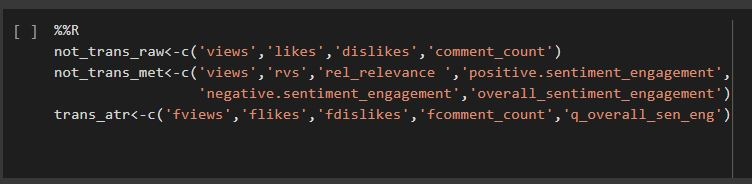
\includegraphics[width=10cm]{col.JPG}
\caption{Divisi\'on de atributos para el c\'alculo de modelos de regresi\'on}
\label{fig:regre}
\end{figure}


\begin{itemize}

\item {\itshape not{\textunderscore}trans{\textunderscore}raw}: Donde se hace uso de los datos en crudo para intentar predecir el n\'umero de {\itshape views}

\item {\itshape not{\textunderscore}trans{\textunderscore}met}: Donde se hace uso de las m\'etricas para intentar predecir el n\'umero de {\itshape views}

\item {\itshape trans{\textunderscore}atr}: Donde se hace uso de los datos transformados para poder predecir el n\'umero de {\itshape views} (transformadas).

\end{itemize}

A continuaci\'on se deja el $85\%$ de los datos para entrenar los modelos, y el resto para hacer el test. Los modelos que se han implementado se pueden ver en la figura \ref{fig:model1}.

\begin{figure}[h!]
\centering
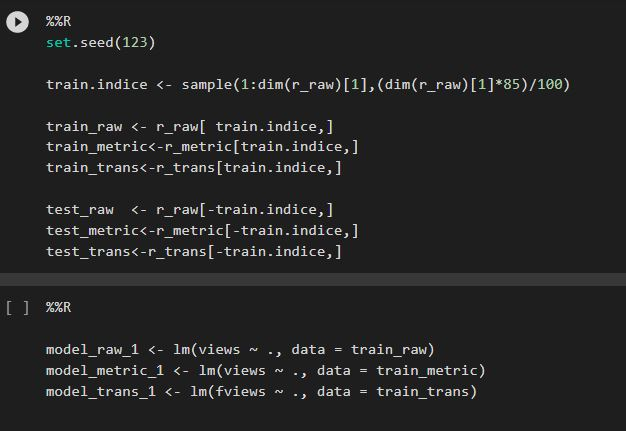
\includegraphics[width=10cm]{modelos_1.JPG}
\caption{Divisi\'on de los datos en train y test e implementaci\'on de modelos}
\label{fig:model1}
\end{figure}

Los volares que obtenemos para $R^{2}$-ajustado son: $0.752$ para {\itshape model{\textunderscore}raw{\textunderscore}1}, 0.001 para  {\itshape model{\textunderscore}metric{\textunderscore}1} y 0.953 para  {\itshape model{\textunderscore}trans{\textunderscore}1}.

A tenor de estos resultados se escoge como mejor modelo: {\itshape model{\textunderscore}trans{\textunderscore}1}. Este modelo usa los atributos que han sufrido una transformaci\'on para que los atributos tengan una distribuci\'on normal. Los atributos tambi\'en presentaban una alta correlaci\'on. Con el fin de otorgar sentido al {\itshape intercept}, tambi\'en se hace el modelo con los datos centrados y escalados. De esta forma el {\itshape intercept} representa el valor de {\itshape fviews} cuando todos los atributos tienen un valor igual a su media. En cualquier caso, el valor de $R^{2}$ ajustado se mantiene constante tanto para el modelo que usa los datos escalados como el que no. Por este motivo mostramos el {\itshape summary} del modelo con los datos escalados y centrados (figura \ref{fig:summ}) .

\begin{figure}[h!]
\centering
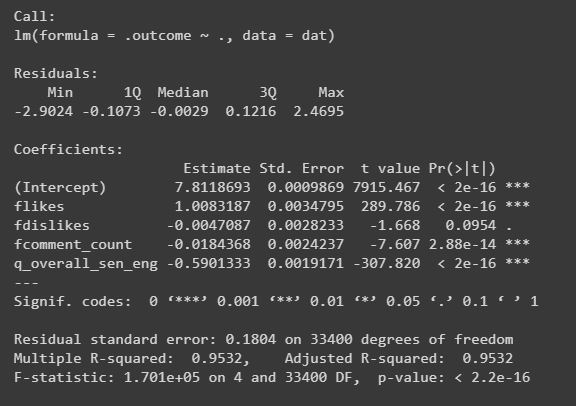
\includegraphics[width=10cm]{summa.JPG}
\caption{Resumen del modelo {\itshape model{\textunderscore}trans{\textunderscore}1}}
\label{fig:summ}
\end{figure}


En la figura  \ref{fig:summ}, se puede ver que el atributo {\itshape fdislikes} no supera el valor t\'ipico para otorgarle relevancia estad\'istica. Por lo que hemos repetido el modelo, pero esta vez sin el atributo {\itshape fdislikes}. Al modelo que cuenta con la variable {\itshape fdislikes} es al que llamamos modelos completo y al modelo que no cuenta con la variable {\itshape fdislikes} lo llamamos reducido. Tanto el modelo completo como el reducido tienen el mismo valor de $R^{2}$ajustado. Con el fin de comprobar formalmente si un modelo es mejor que otro se ha hecho una prueba {\itshape anova} sobre ambos modelos (figura \ref{fig:anov}).

\begin{figure}[h!]
\centering
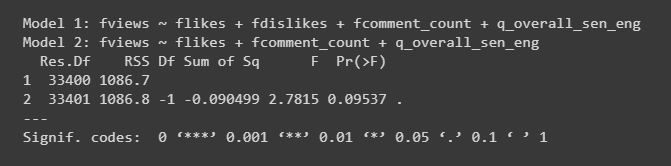
\includegraphics[width=10cm]{anova_modelos.JPG}
\caption{Anova sobre el modelo completo y el reducido}
\label{fig:anov}
\end{figure}

En la figura \ref{fig:anov} se puede ver que el valor de p es lo suficientemente alto como para no poder rechazar la hip\'otesis nula. Por lo no podemos decir que los dos modelos sean diferentes. En este caso elegimos el modelo reducido ya que tienen menos variables y nos ofrecer\'a los mismo resultados.

Por \'ultimo hemos querido comprobar la capacidad predictiva de nuestros modelos, y se ha calculado el valor RMSE (desviaci\'on de m\'inimos cuadrdos), tanto para el modelo de datos en crudo como para el modelo reducido (que usa los atributos transformados), sobre sus respectivos {\itshape test sets}. Adem\'as con el fin de poder establecer una comparaci\'on entre ambos valores el valor de RMSE se ha dividido por los respectivos valores m\'aximos de {\itshape views} y {\itshape fviews} de los {\itshape test sets}.

Para el caso del modelo con datos en crudo hemos encontrado un valore de RMSE de $925483$ y al dividirlo por su m\'aximo $19972$ (la desviaci\'on es casi 20000 mayor que la propia medida). 

Para el modelo reducido tenemos un RMSE de $0.1830192$ y al dividirlo por el valor m\'aximo $0.0553140$. El hecho de que el valor relativo sea menor que uno ya es indicativo que la desciaci\'on es inferior a la medida.  

\subsubsection{M\'etodo 3: Pruebas de contraste de hip\'otesis}

En este punto nos preguntamos que conjunto de categor\'ias de v\'ideos tienen medias de n\'umero de visualizaciones similares estad\'isticamente (no se puede rechazar la hip\'otesis nula). Una forma de comprobar esto es realizar comprobaciones por pares (hecho en el c\'odigo del notebook), sin embargo, tal y como recoge el material que proporciona la UOC para la asignatura de estad\'istica avanzada corremos el riesgo de aceptar alg\'un resultado significativo incluso cuando todos no lo son. Una las alternativas que se proponen es usar una correcci\'on conservadora (Bonferroni). El paquete {\itshape agricolae} que implementa esta correci\'on tiene adem\'as la ventaja que ya nos codifica con las mismas letras los grupos para los que no existe diferencia. En la figura \ref{fig:Berro} se puede ver el resultado para Mexico (aunque en el c\'odigo del notebook est\'an los resultados para todos los pa\'ises).

\begin{figure}[h!]
\centering
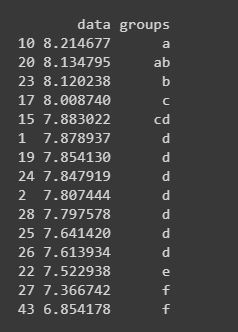
\includegraphics[width=6cm]{Berro.JPG}
\caption{Agrupaci\'on de categorias similares codificadas por letras para Mexico}
\label{fig:Berro}
\end{figure}

\section{Representaci\'on de los resultados a partir de tablas y gr\'aficas.}


\subsection{Cu\'anto tarda un video en llegar a Trending}

Como ya hemos apuntado en la secci\'on sobre el tratamiento de {\itshape outliers}, m\'as del $95\%$ de los v\'ideos llegan a {\itshape trending} en los primeros 40 d\'ias. Con el fin de poder visualizar m\'as claramente  los deltas de tiempo, en la figura \ref{fig:tiempo_2} mostramos como hemos dividido los v\'ideos en intervalos de tiempo seg\'un si tardan entre [0 , 1], (1,2], (2,5], (5,7], (7, 10] (10, 15], (15,30] y (30, 40] d\'ias en llegar a {\itshape trending}. Luego hemos calculado el porcentaje de los v\'ideos con respecto al total.

\begin{figure}[h!]
\centering
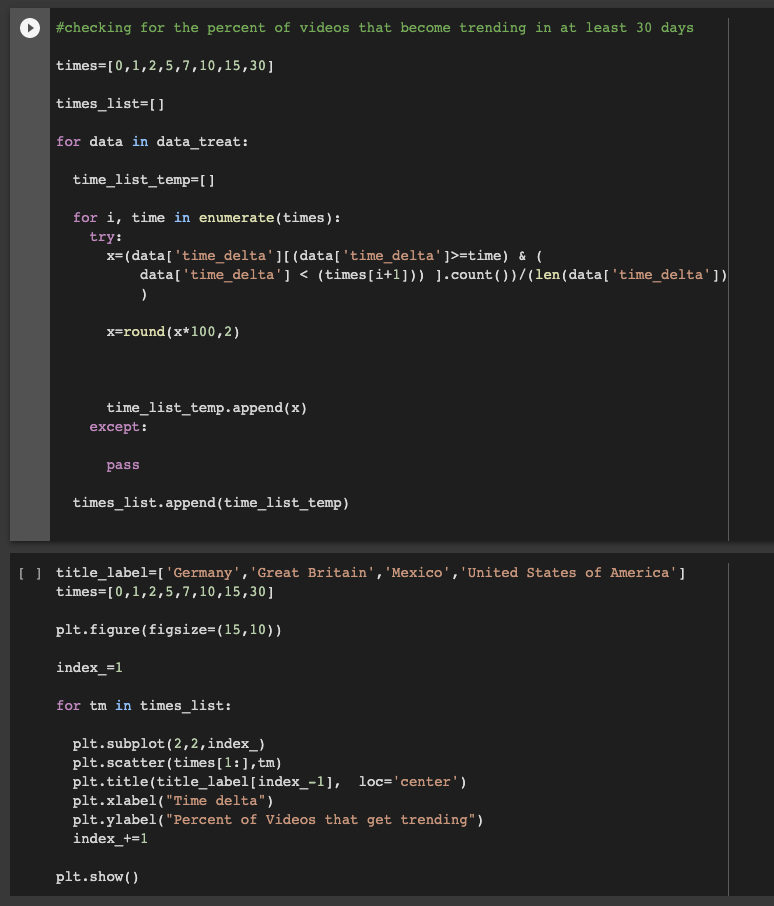
\includegraphics[width=13cm]{plot_freq_code.png}
\caption{Implementaci\'on de la divisi\'on del tiempo en intervalos y c\'alculo de porcentaje}
\label{fig:tiempo_2}
\end{figure}



Los datos mostrados representanen la figura \ref{fig:tiempo_3}  un 98\% de los videos. Estos resultados son muy interesantes ya que nos dan una idea de cuando tarda algo en hacerse popular en un los diferentes paises, cada cuanto utilizan la plataforma los usuarios en los diferentes paises, o cuanto tarda un usuario en ver algo fuera de sus intereses habituales. Por ejemplo en Gran Breta\~na es razonable esperar que un v\'ideo puedo tardar hasta 30 d\'ias en hacerse {\itshape trending}. Para Alemania y Mexico, si el v\'ideo no se ha hecho {\itshape trending} en cinco d\'ias, sus posibiliades de llegar a {\itshape a trending} caen r\'apidamente.

\begin{figure}[h!]
\centering
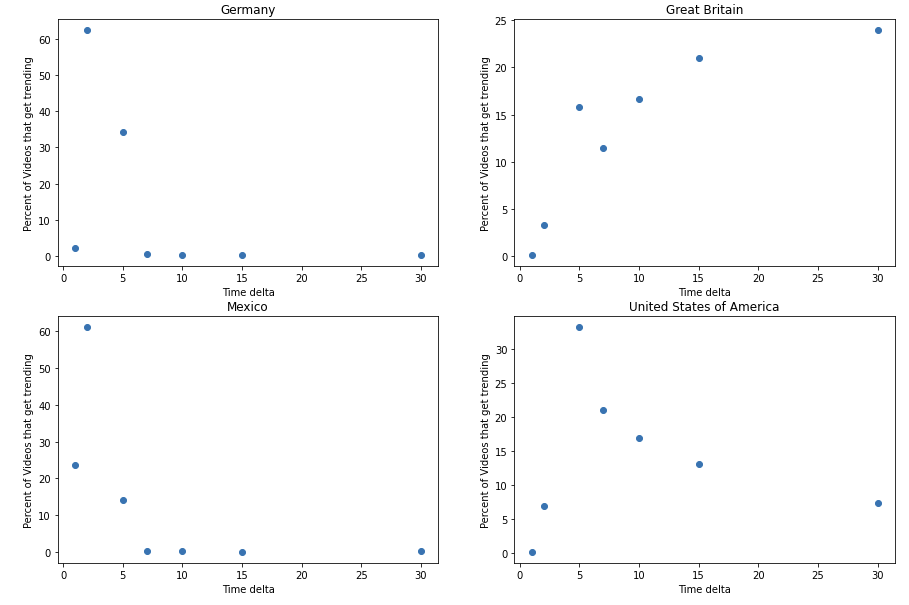
\includegraphics[width=13cm]{plot_freq_perc.png}
\caption{Intervalos de tiempo y porcentaje de v\'ideos}
\label{fig:tiempo_3}
\end{figure}



\subsection{Qu\'e categor\'ias tienen m\'as \'exito en cada pa\'is}

Para realizar visualizaciones correctas sobre las categorias de los videos, vamos crear una columna con el nombre de la categor\'ia del video (ahora mismo solo teniamos sus ids).
\\
\\
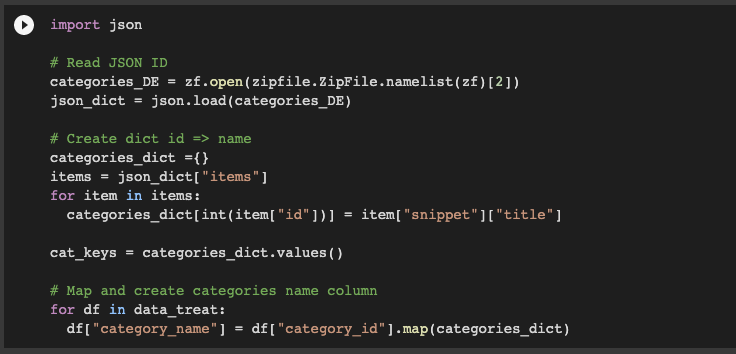
\includegraphics[width=13cm]{categories_1.png}
\\
\\
Una vez tenemos la columna creada, vamos a obtener el numero total de videos en trending por categoria en cada mercado.
\\
\\
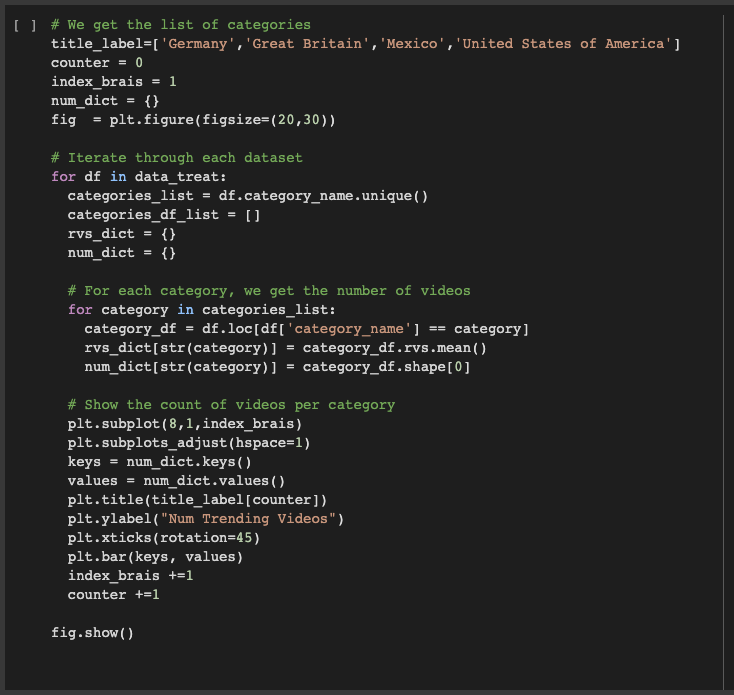
\includegraphics[width=13cm]{categories_2.png}
\\
\\
Con este plot vamos a ser capaces de ver la distribucion de las vistas por cada categoria. Como datos mas relevantes que se pueden observar, los videos de categor\'ia entretenimiento son los que suelen alcanzar trending con m\'as asiduidad.
\\
\\
Otro dato que me ha parecido muy interesante es como los videos musicales son muy populares en EEUU y UK, mientras que en Mejico o Alemania no son casi relevantes.\'Esta informaci\'on podr\'ia ser de gran utilidad para artistas que intentan crecer en diferentes regiones o mercados.
\\
\\
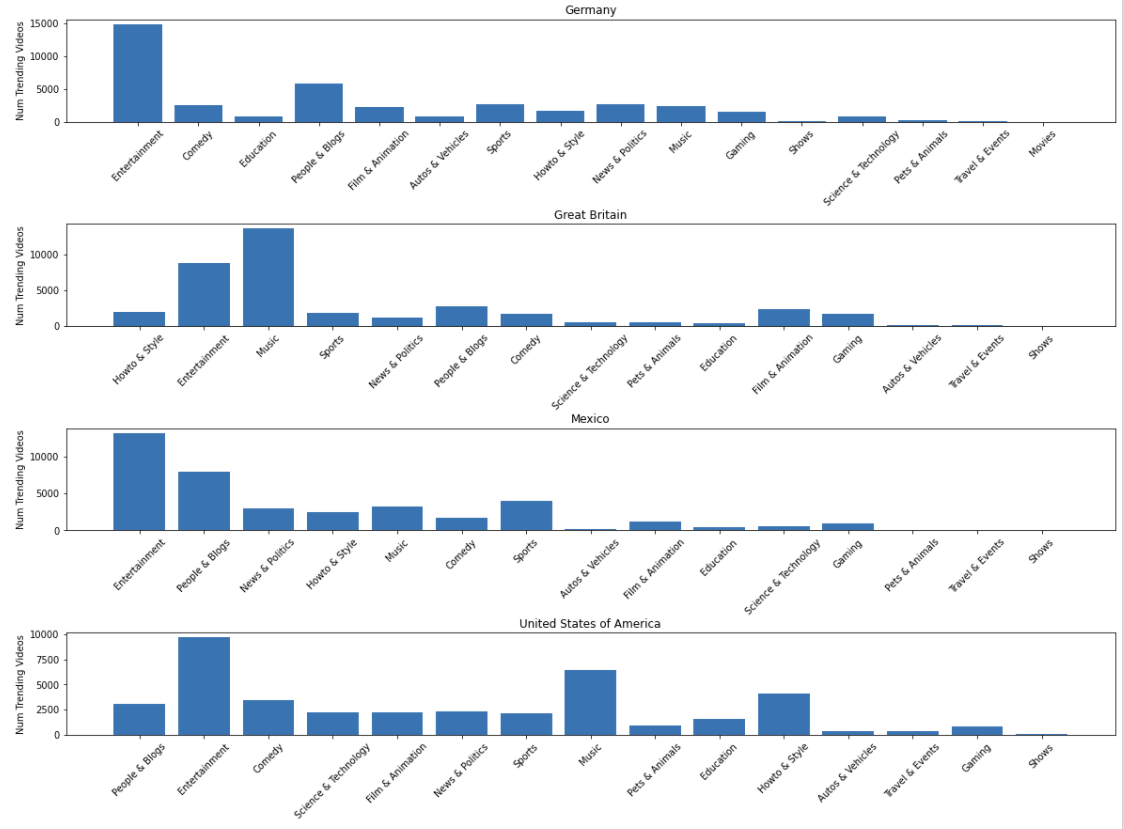
\includegraphics[width=13cm]{plot_categories.png}

\subsection{NLP}

Con el fin de no sobrecargar el trabajo hemos eliminado del ejercicio escrito el c\'alculo de las 50 palabras m\'as relevantes  para cada atributo. As\'i como el an\'alisis de sentimiento para los t\'itulos y el de polaridad. Sin embargo todo el proceso est\'a detallado en el notebook en el apartado {\itshape some NLP}. 
Cabe destacar que hemos encontrado varios problemas en an\'alisis de los textos del dataset Alem\'an. Esto se debe a que en Aleman\'ia hay una fuerte componente de inmigraci\'on turca, y muchos v\'ideos tienen t\'itulos, comentarios y tags en turco, eso \'unido a la pobre codificaci\'on del texto de base y que no entendemos turco nos dificulta extraer resultados satisfactorios del dataset alem\'an.

\subsubsection{Worcloud de n-gramas}

A trav\'es del an\'alisis del {\itshape document-term Matrix} y utilizando el c\'odigo que se presenta en la figura \ref{fig:colud_1}  hemos podido extraer {\itshape word clouds} con sentido para los atributos de texto de cada pa\'is.


\begin{figure}[h!]
\centering
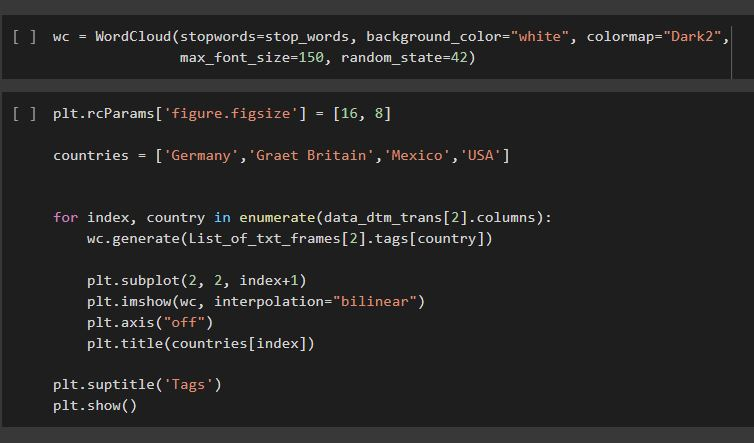
\includegraphics[width=13cm]{cod_word.JPG}
\caption{C\'odigo para generar las {\itshape word clouds}}
\label{fig:colud_1}
\end{figure}

Las \textbf{tags} se pueden ver en la figura \ref{fig:colud_2}.


\begin{figure}[h!]
\centering
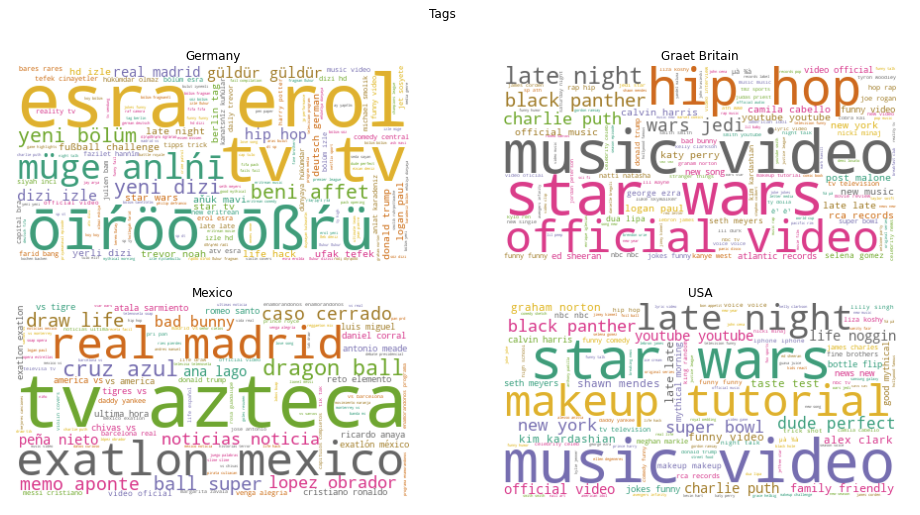
\includegraphics[width=13cm]{wordcloud_tags.png}

\caption{{\itshape Word clouds} para el atributo tag por pa\'is}
\label{fig:colud_2}
\end{figure}

Destacar en el Mexicano, que podemos ver la TV Azteca y exatlon, que es un programa de gran \'exito en el pais (de TV Azteca). En usa parece que {\itshape makeup tutorial} es importante. On Gran Breta\~na {\itshape Star Wars} o {\itshape Black panther} (en este momento cabe destacar que estos datos son del 2017)

Los \textbf{t\'itulos} de los v\'ideos los podemos ver la figura \ref{fig:colud_3}.  



\begin{figure}[h!]
\centering
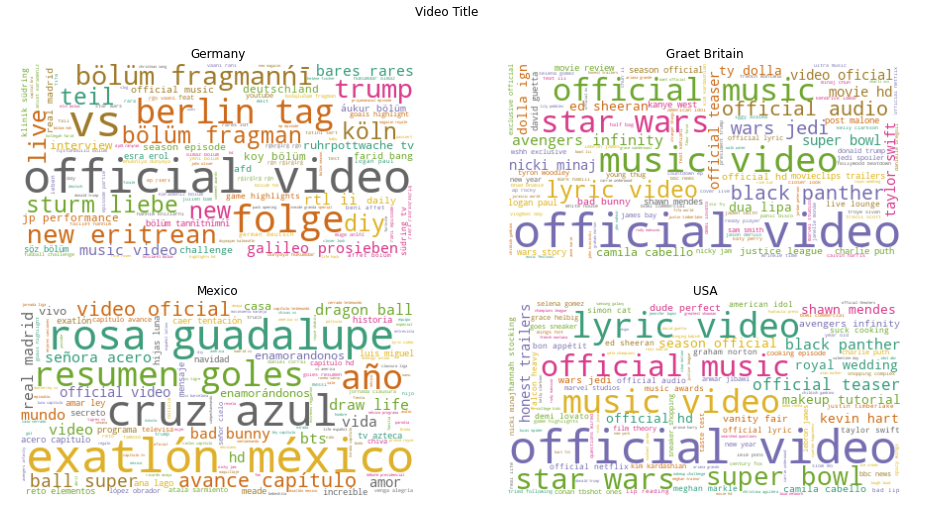
\includegraphics[width=13cm]{wordcloud_title.png}
\caption{{\itshape Word clouds} para el atributo t\'itulo por pa\'is}
\label{fig:colud_3}
\end{figure}

A destacar que la palabra Trump aparece m\'as en lo t\'itulos de Alemania que en EEUU. Los v\'ideos musicales parecen ser muy populares. Los v\'ideos de f\'utbol y otros deportes son mucho mas populares en M\'exico que en el resto de pa\'ises. Los vengadores y Star Wars tienen bastante impacto en UK y EEUU.

Por \'ultimo, en la figura \ref{fig:colud_4},  mostramos las palabras mas utilizadas en las \textbf{descripciones} de los videos.

\begin{figure}[h!]
\centering

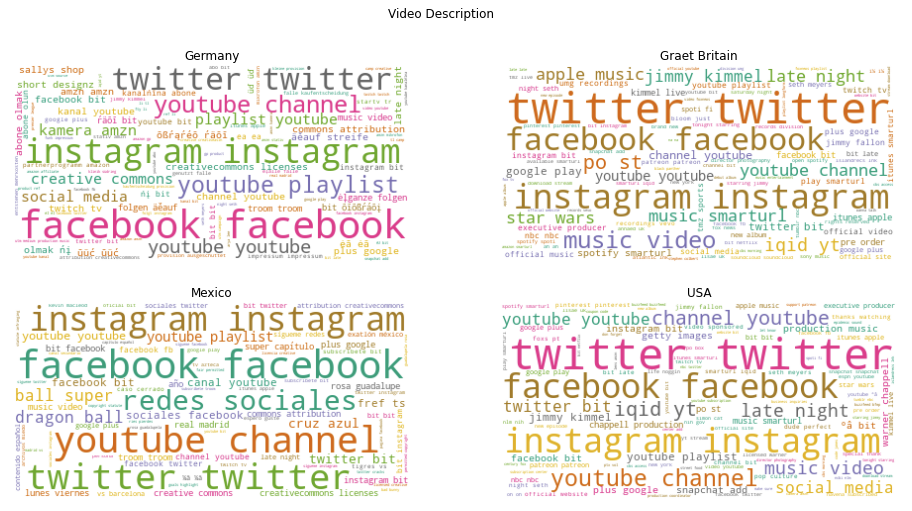
\includegraphics[width=13cm]{wordcould_desc.png}
\caption{{\itshape Word clouds} para el atributodescripci\'on  por pa\'is}
\label{fig:colud_4}
\end{figure}

Como se puede observar, lo que mas se ven son nombres de redes sociales y webs, esto se debe a que la mayor\'ia de creadores de contenido introducen sus redes sociales en la descripci\'on. Para poder obtener informaci\'on relevante de \'esta wordcloud necesitamos realizar m\'as tareas de limpieza.

\subsubsection{Uso de vocabulario}
Una de las cuestiones que nos planteábamos al presentar los objetivos de la pr\'actica es si pod\'iamos encontrar diferencias en el uso del vocabulario de dos pa\'ises donde se hable la misma lengua.

Para realizar este an\'alisis se han contado todas las palabras que al menos ocurren una vez en el {\itshape document term Matrix} de los datasets de Gran Breta\~na y EEUU. Como podemos ver en la figura \ref{fig:voc} de la izquierda en ambos pa\'ises se usan la misma cantidad de palabras \'unicas. Sin embargo cuando nos preguntamos por la diversidad del vocabulario, es decir, en que pa\'is se usa una variedad m\'as amplia de palabras vemos que la diferencia entre Gran Breta\~na y EEUU es bastante notable. En EEUU hay muchas m\'as palabras que aparecen m\'as e 100 veces, por lo que el vocabulario de EEUU se encuentra m\'as concentrado en un n\'umero de palabras m\'as reducido que si lo comparamos con el vocabulario de Gran Breta\~na (figura \ref{fig:voc} derecha). 


\begin{figure}[h!]
\centering

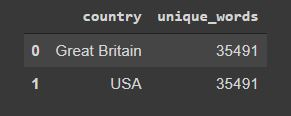
\includegraphics[width=5cm]{coc_comp.JPG}
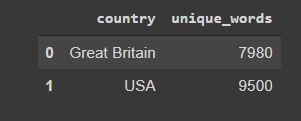
\includegraphics[width=5cm]{dif_voc.JPG}
\caption{Diferencias en vocabulario}
\label{fig:voc}
\end{figure}

\section[item_conclusiones]{Resoluci\'on del problema. A partir de los resultados obtenidos, ?`cu\'ales son las conclusiones? ?`Los resultados permiten responder al problema?}

Siguiendo el esquema de preguntas que nos plante\'abamos al principio de la pr\'actica:
\begin{itemize}

\item  ?` qu\'e categorias son mas populares en cada mercado? Aqu\'i adem\'as de decir que categorias son mas relevantes tambien puedes decir cuales son estad\'isticamnete similares

\item ?` cu\'anto tarda un video en hacerse Trending?
\begin{itemize}
\item depende fuertemente el pa\'is. De los pa\'ises investigados hasta 30 d\'ias es razonable para Gran Breta\~na. Para el resto, despu\'es de cinco d\'ias de su publicaci\'on la cantidad de v\'ideos que llegan a {\itshape a trending se reduce exponencialmente}
\end{itemize}
\item ?`Cuales son las palabras m\'as utilizadas?
\begin{itemize}
\item Aunque no est\'a incluido en el texto si en el c\'odigo. Se han generado diccionarios con las 50 palabras m\'as utilizadas para los distintos atributos de texto de cada pa\'is. Como curiosidad la palabra que m\'as aparece en los t\'itulos de Gran Breta\~na es Tyron: profesional Americano de artes marciales mixtas y comentarista deportivo.
\end{itemize}
\item ?`Cuales son las tags m\'as relevantes?
\begin{itemize}
\item Cabe destacar {\itshape makeup tutorial} para EEUU por lo singular de la tag.
\item De forma general para Gran Breta\~na y EEUU {\itshape Star Wars}, videos musicales, {\itshape Super bowl} y temas relacionados con los Vengadores
\item para Mexico principalmente Tv azteca o Real Madrid  
\end{itemize}
\item ?`Cuales son las temas m\'as importantes?
\begin{itemize}
\item Cine en especial las dos franquicias mencionadas.
\item M\'usica en especial hip hop y v\'ideos musicales
\item Deportes
\item Tambi\'en se pueden ver otros temas que van desde pol\'itica a dragon Ball .
\end{itemize}
\item ?`Existen diferencias en el vocabulario que se utilizan los pa\'ises que hablan la misma lengua?
\begin{itemize}
\item Si, en EEUU el vocabulario se encuentra concentrado en n\'umero m\'as reducido de palabras si lo comparamos con el caso de Gran Breta\~na.
\end{itemize}

\item ?`Cual es el sentimiento y la polaridad expresada en los t\'itulos?
\begin{figure}[h!]
\centering

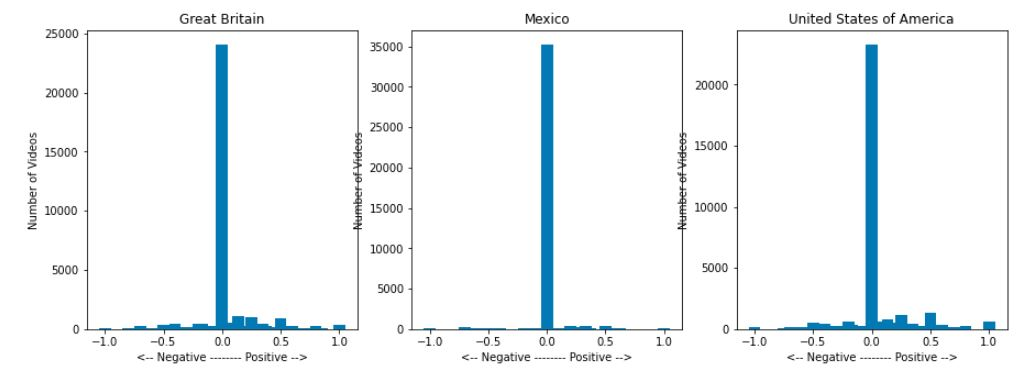
\includegraphics[width=10cm]{Sent.JPG}
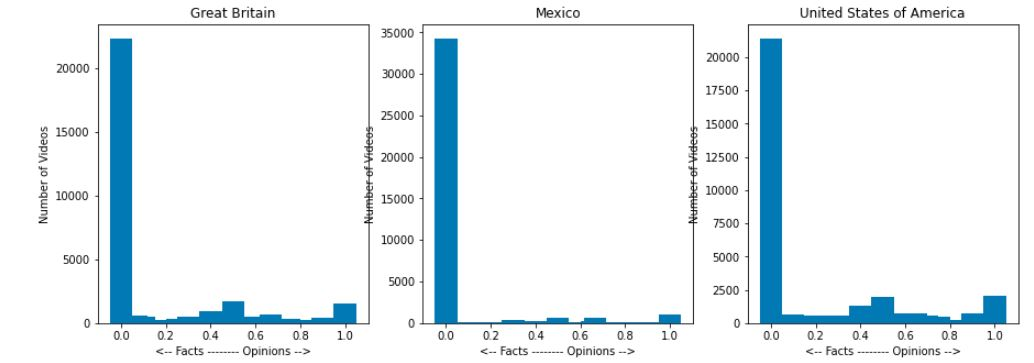
\includegraphics[width=10cm]{pol.JPG}
\caption{Sentimiento arriba, polaridad abajo}
\label{fig:sentpol}
\end{figure}
\begin{itemize}
\item Como se puede ver en la figura \ref{fig:sentpol}, los t\'itulos de los v\'ideos que llegan a {\itshape trending} suelen describir hechos y expresan un sentimiento en su mayor\'ia neutro.
\end{itemize}
\item ?`Podemos modelar en n\'umero de veces que un v\'ideo se ve y establecer un modelo predictivo?

\begin{itemize}

\item Si, aunque un estudio en m\'as detalle ser\'ia necesario
\end{itemize}
\end{itemize}

Hemos obtenido m\'ultiples conclusiones muy interesantes, hemos visto c\'omo los diferentes pa\'ises interact\'uan con los videos, ya sea desde el punto de vista de como reaccionan a ellos o cu\'ales son los m\'as populares.
\\
\\
Todas estas conclusiones ser\'an de gran utilidad para cualquier creador de contenido que trate de hacerse un hueco en YouTube, o incluso grandes empresas que quieran realizar propuestas de marketing a trav\'es de la plataforma podri\'ian utilizar \'esta informaci\'on para especializar los anuncios por comunidad o mercado.


\begin{thebibliography}{9}

\bibitem{td1} Leonard Berzkowitz,%
	\emph{ Advances in Experimental Social Psychology}, 1967,  Academic press
\bibitem{td2} Richard McElreath, Robert Boyd,%
	\emph{ Mathematical Models of Social Evolution: A Guide for the Perplexed}, 2007, The University of Chicago Press
\bibitem{td3}Thomas L. Saaty and Joyce M. Alexander,%
	\emph{Thinking with models: Mathematical Models in the Physical, Biological, and Social Sciences}, 2015, RWS Publications
\bibitem{dd1}Jason Radford and Kenneth Joseph,%
	\emph{Theory In, Theory Out: The Uses of Social Theory in Machine Learning for Social Science}, 2020, doi.org/10.3389/fdata.2020.00018

\end{thebibliography}

\end{document}
